\documentclass[11pt]{article}

% ----- Mandatory Packages -----
\usepackage{amsmath}
\usepackage{amssymb}
\usepackage{amsthm}
\usepackage{geometry}
\usepackage{tikz}
\usetikzlibrary{arrows.meta, positioning, shapes, intersections, backgrounds}
\usepackage{mathrsfs}
\usepackage{mathtools}
\usepackage{enumitem}
\usepackage{xcolor}

% ----- Page Setup -----
\geometry{
    a4paper,
    left=1in,
    right=1in,
    top=1in,
    bottom=1in
}

% ----- Theorem Environments -----
\newtheorem{theorem}{Theorem}[section]
\newtheorem{lemma}[theorem]{Lemma}
\newtheorem{corollary}[theorem]{Corollary}
\newtheorem{proposition}[theorem]{Proposition}
\theoremstyle{definition}
\newtheorem{definition}[theorem]{Definition}
\newtheorem{example}[theorem]{Example}
\newtheorem{problem}{Problem}
\newtheorem{axiom}{Axiom}
\theoremstyle{remark}
\newtheorem{remark}[theorem]{Remark}

% ----- Custom Macros -----
\newcommand{\E}{\mathbb{E}}
\newcommand{\R}{\mathbb{R}}
\newcommand{\Prob}{\mathbb{P}}
\newcommand{\Var}{\text{Var}}
\newcommand{\F}{\mathcal{F}}
\newcommand{\samplemean}{\bar{y}}

% ----- Metadata -----
\title{\textbf{Homework 1: Introduction to Statistical Theory}}
\author{Tashfeen Omran}
\date{September 2026}

\begin{document}

\maketitle
\tableofcontents
\newpage

% ======================================================================
% PART 1: Comprehensive Introduction, Context, and Prerequisites
% ======================================================================
\section{Part 1: Comprehensive Introduction, Context, and Prerequisites}

\subsection{Historical Context and Motivation}
Historically, mathematical statistics evolved from empirical observation to a highly rigorous subfield of probability theory. Early probabilists like Laplace and Gauss investigated errors in astronomical observations, leading to the formulation of the Gaussian distribution. However, the foundational crisis of the 19th and early 20th centuries demanded absolute rigor. It was Andrey Kolmogorov in 1933 who provided the axiomatic foundations of probability via measure theory. This framework allowed statisticians to formally bridge the gap between empirical samples (the data we observe) and theoretical populations (the abstract probability spaces generating the data). Statistics, therefore, is not mere accounting; it is the mathematical science of inference, allowing us to approximate abstract, infinitely large functional spaces using finite subsets governed by rigorous probability bounds.

\subsection{Core Concepts \& Axioms}
The essence of statistical theory is inference: inferring the properties of a measurable space from a finite realization of random variables. 
\begin{itemize}
    \item \textbf{Probability Space:} We denote a probability space as a triplet $(\Omega, \F, \Prob)$, where $\Omega$ is the sample space (the population), $\F$ is a $\sigma$-algebra of measurable subsets of $\Omega$ (events), and $\Prob$ is a probability measure such that $\Prob(\Omega) = 1$.
    \item \textbf{Random Variable:} A real-valued random variable $Y$ is an $\F$-measurable function $Y: \Omega \to \R$. 
    \item \textbf{Population vs. Sample:} The \textit{population} corresponds to the complete probability space $(\Omega, \F, \Prob)$ or the full distribution of the random variable $Y$. A \textit{sample} $y_1, y_2, \dots, y_n$ is a finite realization of independent and identically distributed (i.i.d.) random variables $Y_1, \dots, Y_n$ drawn from $\Omega$.
    \item \textbf{Statistic:} A statistic is any measurable function of the sample data, $T(Y_1, \dots, Y_n)$, which does not depend on unknown parameters.
\end{itemize}

\subsection{Intuition and Set-Theoretic/Logical Foundations}
When we compute a relative frequency histogram, we are essentially constructing an \textit{empirical probability measure} $\Prob_n$. By partitioning the range of data into disjoint Borel sets (intervals) $A_j$, we evaluate $\Prob_n(A_j) = \frac{1}{n} \sum_{i=1}^n \mathbf{1}_{A_j}(y_i)$, where $\mathbf{1}$ is the indicator function. The Glivenko-Cantelli theorem, a cornerstone of probability, ensures that as $n \to \infty$, the empirical measure converges to the true probability measure $\Prob(A_j)$. Density curves are merely the Radon-Nikodym derivatives of these absolutely continuous probability measures with respect to the Lebesgue measure.

\subsection{Key Theorems, Lemmas, and Formulas}
\begin{enumerate}
    \item \textbf{Linearity of Finite Sums:} Given constants $c$, sequences $x_i, y_i$:
    \[ \sum_{i=1}^n c = nc, \quad \sum_{i=1}^n c y_i = c \sum_{i=1}^n y_i, \quad \sum_{i=1}^n (x_i + y_i) = \sum_{i=1}^n x_i + \sum_{i=1}^n y_i \]
    \item \textbf{Sample Mean (First Moment of empirical measure):} 
    \[ \samplemean = \frac{1}{n} \sum_{i=1}^n y_i \]
    \item \textbf{Sample Variance (Unbiased Estimator for Second Central Moment):}
    \[ s^2 = \frac{1}{n-1} \sum_{i=1}^n (y_i - \samplemean)^2 \]
    \item \textbf{The Empirical Rule (Gaussian Measure Bounds):} If $Y \sim \mathcal{N}(\mu, \sigma^2)$, then:
    \[ \Prob(|Y - \mu| \le \sigma) \approx 0.68, \quad \Prob(|Y - \mu| \le 2\sigma) \approx 0.95, \quad \Prob(|Y - \mu| \le 3\sigma) \approx 0.997 \]
\end{enumerate}

\subsection{Prerequisites}
To fully synthesize this material, the reader must possess a solid foundation in:
\begin{itemize}
    \item \textit{Set Theory:} Understanding partitions, unions, and intersections.
    \item \textit{Basic Real Analysis:} Summation limits, integrals as areas under curves.
    \item \textit{Algebraic Manipulation:} Distributive properties over finite summation operators.
\end{itemize}

% ======================================================================
% PART 2: Detailed Homework Solutions
% ======================================================================
\section{Part 2: Detailed Homework Solutions (Rigorous Proofs \& Computations)}

\begin{problem}[Example 1 - Population and Sample Definitions]
The voltage at a particular point in the guidance system for a spacecraft may be tested in the only three systems that have been built. The resulting data could be used to estimate the voltage characteristics for other systems that might be manufactured some time in the future. What is the population and the sample?
\end{problem}
\begin{proof}[Solution Setup and Logical Deduction]
By definition, a sample $S$ is a finite subset of a population $P$, strictly formally $S \subset P$. The population $P$ encompasses the entire target group of interest for inference making.
\begin{enumerate}
    \item The problem states we want to "estimate... characteristics for other systems that might be manufactured some time in the future." Therefore, the population is the theoretically infinite set of all potential systems to be built under these specifications.
    \item The sample is the specific set of elements drawn from the population for which we possess measured data. Here, only 3 systems have been built and tested.
\end{enumerate}
\textbf{Conclusion:} 
The sample is the $3$ guidance systems that have been built. 
The population is the set of \textit{all potential} guidance systems to be built.
\end{proof}

\begin{problem}[Example 2 - Histogram Construction]
Construct a relative frequency histogram with an interval width of $0.2$, starting at $2.05$, for the following data set:
$\{2.1, 2.2, 2.3, 2.4, 2.4, 2.5, 2.6, 2.6, 2.7, 2.9\}$.
\end{problem}
\begin{proof}[Computation and Setup]
Let our dataset be indexed as $y_1, y_2, \dots, y_{10}$. The sample size is $n=10$. We are partitioning the measurable space into right-open, left-closed intervals (Borel sets) of the form $I_k = [a_k, b_k)$ with width $b_k - a_k = 0.2$. The relative frequency for $I_k$ is the empirical measure $\Prob_n(I_k) = \frac{1}{n}\sum_{i=1}^{10} \mathbf{1}_{I_k}(y_i)$.
\begin{itemize}
    \item $I_1 = [2.05, 2.25)$: $y \in \{2.1, 2.2\}$. Count $= 2$. Relative Frequency $= 2/10 = 0.2$.
    \item $I_2 = [2.25, 2.45)$: $y \in \{2.3, 2.4, 2.4\}$. Count $= 3$. Relative Frequency $= 3/10 = 0.3$.
    \item $I_3 = [2.45, 2.65)$: $y \in \{2.5, 2.6, 2.6\}$. Count $= 3$. Relative Frequency $= 3/10 = 0.3$.
    \item $I_4 = [2.65, 2.85)$: $y \in \{2.7\}$. Count $= 1$. Relative Frequency $= 1/10 = 0.1$.
    \item $I_5 = [2.85, 3.05)$: $y \in \{2.9\}$. Count $= 1$. Relative Frequency $= 1/10 = 0.1$.
\end{itemize}
The sum of relative frequencies is $0.2 + 0.3 + 0.3 + 0.1 + 0.1 = 1.0$, which satisfies the second axiom of probability (unit measure). 
\end{proof}

\begin{problem}[Summation Property Proofs]
Prove the following properties for a sample of $n$ observations $y_1, \dots, y_n$ and constant $c$: \\
1. $\sum_{i=1}^n c = nc$ \quad 2. $\sum_{i=1}^n c y_i = c \sum_{i=1}^n y_i$ \quad 3. $\sum_{i=1}^n (x_i + y_i) = \sum_{i=1}^n x_i + \sum_{i=1}^n y_i$
\end{problem}
\begin{proof}[Proof of Summation Properties]
We use direct proofs relying on the algebraic axioms of real numbers (associativity, commutativity, and distributivity).
\begin{itemize}
    \item \textbf{Proof 1:} By definition of summation, $\sum_{i=1}^n c = c + c + \dots + c$ (where $c$ is added $n$ times). By the definition of multiplication over the integers, this is strictly $nc$.
    \item \textbf{Proof 2:} By definition, $\sum_{i=1}^n c y_i = c y_1 + c y_2 + \dots + c y_n$. By the distributive property of multiplication over addition in $\R$, we can factor out the scalar $c$, yielding $c (y_1 + y_2 + \dots + y_n)$, which is $c \sum_{i=1}^n y_i$.
    \item \textbf{Proof 3:} By definition, $\sum_{i=1}^n (x_i + y_i) = (x_1 + y_1) + (x_2 + y_2) + \dots + (x_n + y_n)$. Because addition in $\R$ is associative and commutative, we can rearrange the terms by grouping the $x$ sequence and the $y$ sequence: $(x_1 + x_2 + \dots + x_n) + (y_1 + y_2 + \dots + y_n)$. This perfectly corresponds to $\sum_{i=1}^n x_i + \sum_{i=1}^n y_i$.
\end{itemize}
This completes the proofs. $\blacksquare$
\end{proof}

\begin{problem}[Example 3 - Summation of Deviations]
Prove that the summation of the deviations of a set of measurements about their mean is equal to zero. That is, prove that $\sum_{i=1}^n (y_i - \samplemean) = 0$.
\end{problem}
\begin{proof}[Direct Algebraic Proof]
Let $y_1, y_2, \dots, y_n$ be elements of $\R$ and define the sample mean as $\samplemean = \frac{1}{n}\sum_{i=1}^n y_i$. 
\begin{align*}
    \sum_{i=1}^n (y_i - \samplemean) &= \sum_{i=1}^n y_i - \sum_{i=1}^n \samplemean \quad &&\text{(By Summation Property 3, additive separation)} \\
    &= \sum_{i=1}^n y_i - n\samplemean \quad &&\text{(By Summation Property 1, since $\samplemean$ is a constant with respect to $i$)} \\
    &= \sum_{i=1}^n y_i - n\left(\frac{1}{n}\sum_{i=1}^n y_i\right) \quad &&\text{(Substituting the definition of the sample mean $\samplemean$)} \\
    &= \sum_{i=1}^n y_i - \sum_{i=1}^n y_i \quad &&\text{(Algebraic simplification: $n \times \frac{1}{n} = 1$)} \\
    &= 0 \quad &&\text{(Property of additive inverses in $\R$)}
\end{align*}
The summation of deviations about the mean strictly maps to the zero element. $\blacksquare$
\end{proof}

\begin{problem}[Example 4 - Calculating Sample Moments]
Using the data set $\{3, 3, 2, 4, 1\}$, calculate the sample mean, sample variance, and sample standard deviation.
\end{problem}
\begin{proof}[Calculation Setup]
The dataset $Y$ has cardinality $n = 5$.
\begin{itemize}
    \item \textbf{Sample Mean:} 
    \[ \samplemean = \frac{1}{n}\sum_{i=1}^n y_i = \frac{1}{5}(3 + 3 + 2 + 4 + 1) = \frac{13}{5} = 2.6 \]
    \item \textbf{Sample Variance ($s^2$):} 
    Using the unbiased estimator $s^2 = \frac{1}{n-1} \sum_{i=1}^n (y_i - \samplemean)^2$.
    \begin{align*}
        \sum_{i=1}^n (y_i - 2.6)^2 &= (3 - 2.6)^2 + (3 - 2.6)^2 + (2 - 2.6)^2 + (4 - 2.6)^2 + (1 - 2.6)^2 \\
        &= (0.4)^2 + (0.4)^2 + (-0.6)^2 + (1.4)^2 + (-1.6)^2 \\
        &= 0.16 + 0.16 + 0.36 + 1.96 + 2.56 \\
        &= 5.2
    \end{align*}
    Therefore, $s^2 = \frac{5.2}{5-1} = \frac{5.2}{4} = 1.3$.
    \item \textbf{Sample Standard Deviation ($s$):}
    The standard deviation is the positive square root of the variance (projecting the measure of dispersion back to the original Euclidean scale):
    \[ s = \sqrt{1.3} \approx 1.1402 \]
\end{itemize}
\textbf{Final Answers:} $\samplemean = 2.6$, $s^2 = 1.3$, $s \approx 1.14$.
\end{proof}

\begin{problem}[Example 5 - Empirical Rule]
Suppose the age of retirement is approximately bell-shaped with a mean age of $64.2$ and a standard deviation of $2.9$. Using the empirical rule:
(a) What percentage of people retire after age 70? 
(b) What percentage of people retire before age 61.3?
\end{problem}
\begin{proof}[Probabilistic Assessment]
Let $X$ represent the age of retirement. The problem posits that $X$ follows an approximately Normal (Gaussian) distribution, $X \sim \mathcal{N}(64.2, (2.9)^2)$. The Empirical Rule (an approximation of the integral of the Gaussian density function) asserts that for bounds $\mu \pm k\sigma$:
$k=1 \implies 68\%$, $k=2 \implies 95\%$, $k=3 \implies 99.7\%$.

\textbf{Part (a):} Determine $\Prob(X > 70)$.
Notice that $70 = 64.2 + (2 \times 2.9) = \mu + 2\sigma$.
Because the Normal distribution is perfectly symmetric around $\mu$, the area outside $\mu \pm 2\sigma$ is $100\% - 95\% = 5\%$.
This $5\%$ is evenly split into the two tails. 
Thus, $\Prob(X > \mu + 2\sigma) = \frac{5\%}{2} = 2.5\%$.

\textbf{Part (b):} Determine $\Prob(X < 61.3)$.
Notice that $61.3 = 64.2 - 2.9 = \mu - 1\sigma$.
The area within $\mu \pm 1\sigma$ is $68\%$. The remaining area outside this interval is $100\% - 68\% = 32\%$.
Due to symmetry, the area exclusively in the lower tail (less than $\mu - \sigma$) is $\frac{32\%}{2} = 16\%$.

\textbf{Conclusion:} (a) $2.5\%$ of people retire after 70. (b) $16\%$ of people retire before 61.3.
\end{proof}

\begin{problem}[Inference Logical Deduction]
Suppose we have an election with Candidate A and Candidate B. Candidate A wins if the population proportion favoring them is above $0.5$. Suppose we take a completely random sample of 20 voters, and all 20 say they'll vote for A. What can we conclude about the population?
\end{problem}
\begin{proof}[Logical Argument setup via Probabilistic Contradiction]
We define our population as all eligible voters in the area who will vote. Let $p$ be the true proportion of voters favoring Candidate A. We wish to test the hypothesis that Candidate A might lose, which logically implies $p \le 0.5$.
If $p \le 0.5$, the probability of selecting 20 consecutive voters favoring A, assuming independent trials, is modeled by a Binomial distribution.
\[ \Prob(X = 20 \mid p \le 0.5) \le (0.5)^{20} \approx 0.00000095 \]
Because this probability measure is infinitesimally small (nearly zero), observing this specific sample realization under the assumption $p \le 0.5$ is extremely unlikely. Therefore, we reject the premise.
\textbf{Conclusion:} If less than $50\%$ of voters plan on voting for Candidate A, this observed sample outcome is not logically impossible, but it is highly unlikely probabilistically. Therefore, we infer with high confidence that Candidate A is favored to win ($p > 0.5$).
\end{proof}


% ======================================================================
% PART 3: In-Depth Analysis of Problems and Techniques
% ======================================================================
\section{Part 3: In-Depth Analysis of Problems and Techniques}

\subsection{A) Problem Types and Logical Strategies}
The problems in this chapter fall strictly into three categories of mathematical reasoning:
\begin{enumerate}
    \item \textbf{Algebraic Manipulations of Summation Operators (Problems 3 \& 4):} The overarching strategy here is exploiting the linearity of summation. These are fundamental existence/equivalence proofs demonstrating that operations performed globally on a series can be decomposed into localized operations. 
    \item \textbf{Measure Construction and Evaluation (Problems 2 \& 5):} This involves projecting raw data onto derived mathematical structures. Creating a histogram is formally equivalent to defining a discrete probability mass function (p.m.f.) from empirical data. The calculation of variance forces the student to map vectors of data into Euclidean distance spaces (squared deviations).
    \item \textbf{Probabilistic Contradiction / Hypothesis Testing (Problem 7):} This relies on the core logic of statistical inference. The strategy is analogous to \textit{reductio ad absurdum} (proof by contradiction) in pure logic. We assume a null state (Candidate A has $\le 50\%$) and show that the observed data leads to a probabilistic absurdity ($\Prob < 10^{-6}$).
\end{enumerate}

\subsection{B) Key Analytical and Logical Manipulations}
\begin{itemize}
    \item \textbf{The "Adding Zero" or "Multiplying by One" Trick:} While not explicitly required in the simple proof of $\sum (y_i - \samplemean) = 0$, algebraic expansions of sample variance heavily rely on the trick of adding and subtracting the mean (a "fancy zero").
    \item \textbf{Leveraging Symmetry (The Empirical Rule):} In Problem 6, we bypassed complex calculus (integrating $e^{-x^2}$) by exploiting the geometric symmetry of the Gaussian density curve. Because the measure $P(X > \mu) = P(X < \mu) = 0.5$, we could determine the measure of the tails by simple arithmetic subtraction from 1. 
    \item \textbf{Bessel's Correction ($n-1$ denominator):} In Problem 5, calculating $s^2$ used $n-1$ instead of $n$. The mathematical necessity for this lies in the fact that calculating $\samplemean$ consumes one degree of freedom. By forcing the deviations to sum to zero (Problem 4 constraint), the vector of deviations $(y_1 - \samplemean, \dots, y_n - \samplemean)$ is restricted to an $(n-1)$-dimensional hyperplane. Dividing by $n$ would systematically underestimate the true population variance (biased estimator).
\end{itemize}


% ======================================================================
% PART 4: "Cheatsheet", Visuals, and Tips for Success
% ======================================================================
\section{Part 4: "Cheatsheet", Visuals, and Tips for Success}

\subsection{Visualizing Probability Measure: The Empirical Rule}
Below is a visual representation of the Gaussian measure space partitioned by standard deviations.

\begin{center}
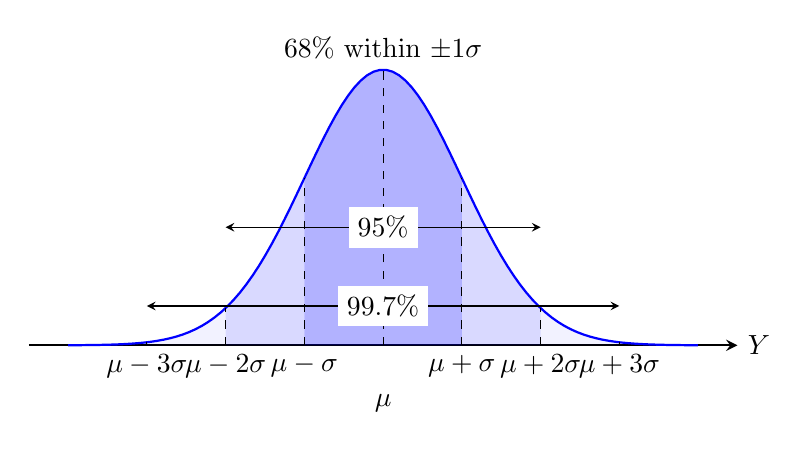
\begin{tikzpicture}
    % Define normal distribution function
    \def\normaltwo#1{3.5*exp(-0.5*(#1)^2)}
    
    % Draw the X axis
    \draw[thick, ->, >=stealth] (-4.5,0) -- (4.5,0) node[right] {$Y$};
    
    % Draw the bell curve
    \draw[thick, domain=-4:4, samples=100, blue] plot (\x, {\normaltwo{\x}});
    
    % Shade 68% (1 std dev)
    \begin{scope}
        \clip (-1,0) rectangle (1,4);
        \fill[blue, opacity=0.3] (-4,0) -- plot[domain=-4:4, samples=100] (\x, {\normaltwo{\x}}) -- (4,0) -- cycle;
    \end{scope}
    
    % Shade 95% (2 std dev)
    \begin{scope}
        \clip (-2,0) rectangle (-1,4);
        \fill[blue, opacity=0.15] (-4,0) -- plot[domain=-4:4, samples=100] (\x, {\normaltwo{\x}}) -- (4,0) -- cycle;
    \end{scope}
    \begin{scope}
        \clip (1,0) rectangle (2,4);
        \fill[blue, opacity=0.15] (-4,0) -- plot[domain=-4:4, samples=100] (\x, {\normaltwo{\x}}) -- (4,0) -- cycle;
    \end{scope}

    % Shade 99.7% (3 std dev)
    \begin{scope}
        \clip (-3,0) rectangle (-2,4);
        \fill[blue, opacity=0.05] (-4,0) -- plot[domain=-4:4, samples=100] (\x, {\normaltwo{\x}}) -- (4,0) -- cycle;
    \end{scope}
    \begin{scope}
        \clip (2,0) rectangle (3,4);
        \fill[blue, opacity=0.05] (-4,0) -- plot[domain=-4:4, samples=100] (\x, {\normaltwo{\x}}) -- (4,0) -- cycle;
    \end{scope}

    % Draw grid lines
    \draw[dashed] (0,0) -- (0,{\normaltwo{0}}) node[above] {$68\%$ within $\pm 1\sigma$};
    \draw[dashed] (-1,0) node[below] {$\mu-\sigma$} -- (-1,{\normaltwo{-1}});
    \draw[dashed] (1,0) node[below] {$\mu+\sigma$} -- (1,{\normaltwo{1}});
    
    \draw[dashed] (-2,0) node[below] {$\mu-2\sigma$} -- (-2,{\normaltwo{-2}});
    \draw[dashed] (2,0) node[below] {$\mu+2\sigma$} -- (2,{\normaltwo{2}});
    \draw[<->, >=stealth] (-2, 1.5) -- (2, 1.5) node[midway, fill=white] {$95\%$};
    
    \draw[dashed] (-3,0) node[below] {$\mu-3\sigma$} -- (-3,{\normaltwo{-3}});
    \draw[dashed] (3,0) node[below] {$\mu+3\sigma$} -- (3,{\normaltwo{3}});
    \draw[<->, >=stealth] (-3, 0.5) -- (3, 0.5) node[midway, fill=white] {$99.7\%$};
    
    \node[below] at (0,-0.5) {$\mu$};
\end{tikzpicture}
\end{center}

\subsection{Heuristics \& "Cheats"}
\begin{itemize}
    \item \textbf{Summation Shortcut:} If you ever see an index variable inside a summation without a subscript $i$, treat it immediately as a constant. Pull it to the front.
    \item \textbf{Variance Translation Check:} Variance is strictly shift-invariant. $\Var(Y_i + C) = \Var(Y_i)$. If you add a constant to all your data points, the variance will not change. You can mentally verify your calculations by shifting large numbers closer to zero before squaring.
\end{itemize}

\subsection{Pitfalls \& Fallacies}
\begin{itemize}
    \item \textbf{The $n$ vs. $n-1$ Trap:} Using $n$ in the denominator calculates the \textit{population} variance $\sigma^2$ under the assumption you have all data. For sample data, you MUST use $n-1$ to prevent a downward bias.
    \item \textbf{Base Rate / Representative Fallacy:} Applying the Empirical Rule to highly skewed data (like income or exponential failure times). The 68-95-99.7 rule is physically invalid for non-Gaussian distributions.
    \item \textbf{Conflating Variance with Standard Deviation:} When comparing spread intuitively, standard deviation is in the same units as the mean. Variance is squared units (e.g., "squared dollars").
\end{itemize}


% ======================================================================
% PART 5: Conceptual Synthesis and The "Big Picture"
% ======================================================================
\section{Part 5: Conceptual Synthesis and The "Big Picture"}

\subsection{A) Thematic Connections}
The core theme of this chapter is \textit{formalizing randomness through functional mapping}. Before this, raw data is simply a chaotic set of numbers. By defining the concepts of sample mean, variance, and relative frequency distributions, we are formally establishing isomorphisms between unstructured real-world phenomena and structured mathematical probability spaces. We summarize chaos into two definitive parameters: expected location (central tendency) and expected entropy/dispersion (variance). 

\subsection{B) Forward and Backward Links}
Backwardly, this material relies on the bedrock of arithmetic and set summation. Forwardly, this is the absolute starting point for advanced analytical probability. 
\begin{itemize}
    \item The sample mean $\samplemean$ sets up the \textbf{Law of Large Numbers (LLN)}, proving that empirical probability measures converge weakly to true probability measures.
    \item The empirical rule is a soft introduction to the \textbf{Central Limit Theorem (CLT)}, which will later prove that the sums of random variables—regardless of their initial distribution—asymptotically converge in distribution to the Gaussian measure $\mathcal{N}(\mu, \sigma^2/n)$.
    \item Understanding summation operators over $\sigma$-algebras prepares the student for advanced Lebesgue integrals used in Stochastic Calculus.
\end{itemize}


% ======================================================================
% PART 6: Abstract Real-World Modeling (AI, ML, & Quant Finance)
% ======================================================================
\section{Part 6: Abstract Real-World Modeling}

\subsection{A) Concrete Scenarios}
In advanced applied mathematics, the foundational theories of statistics act as the mechanical gears driving complex models:
\begin{enumerate}
    \item \textbf{Quantitative Finance (Stochastic Volatility):} In the Black-Scholes-Merton model for derivative pricing, the sample variance of log-returns from historical data is calculated precisely using the summation formulas derived in this chapter. This empirical variance is used to estimate the instantaneous diffusion coefficient ($\sigma$) in geometric Brownian motion.
    \item \textbf{Machine Learning (Empirical Risk Minimization):} In Statistical Learning Theory, the goal of a neural network is to minimize the expected risk (true population loss). However, because the population distribution of data is unknown, the algorithm minimizes the \textit{empirical risk} (the sample mean of the loss function over the training data). The bounds between sample loss and population loss are derived using the variance of the model's hypotheses.
\end{enumerate}

\subsection{B) Model Problem Setup: Algorithmic Trading \& Brownian Motion}
\textit{Objective:} Model the continuous-time price evolution of an asset $S_t$ using empirical statistics.

Let $(\Omega, \F, \Prob)$ be a probability space with a standard Wiener process $W_t$. The state space of the asset price is strictly positive, $S_t \in \R_{>0}$. 
We observe a discrete \textit{sample} of daily closing prices $S_0, S_1, \dots, S_n$. 
First, we construct the log-returns, mapping our data to a stationary process:
\[ y_i = \ln\left(\frac{S_i}{S_{i-1}}\right) \quad \text{for } i = 1, \dots, n \]
By standard statistical theory, we estimate the drift parameter (expected value) and the volatility squared (variance):
\[ \hat{\mu}_{\text{emp}} = \frac{1}{n}\sum_{i=1}^n y_i, \quad \hat{\sigma}^2_{\text{emp}} = \frac{1}{n-1}\sum_{i=1}^n (y_i - \hat{\mu}_{\text{emp}})^2 \]
Using these empirical estimators drawn directly from our sample statistics, we construct the stochastic differential equation (SDE) governing the continuous asset path:
\[ dS_t = \left( \frac{\hat{\mu}_{\text{emp}}}{\Delta t} + \frac{1}{2}\frac{\hat{\sigma}^2_{\text{emp}}}{\Delta t} \right) S_t \, dt + \left( \frac{\hat{\sigma}_{\text{emp}}}{\sqrt{\Delta t}} \right) S_t \, dW_t \]
Here, Ito's Lemma enforces the addition of $\frac{1}{2}\sigma^2$ to the drift term to maintain martingale conditions under the risk-neutral measure $\mathbb{Q}$. This is an advanced extension proving why accurate, unbiased sample variance computation ($n-1$) is critical: biased inputs here will catastrophically misprice options.


% ======================================================================
% PART 7: Common Variations and Untested Concepts
% ======================================================================
\section{Part 7: Common Variations and Untested Concepts}

The provided homework exclusively tests the definitional formula of sample variance and relies on the Empirical Rule for Gaussian data. Standard university curricula always introduce the \textbf{Algebraic (Computational) Formula for Variance} and \textbf{Chebyshev's Inequality} (for non-Gaussian distributions).

\subsection{Missing Concept 1: The Algebraic Variance Formula}
\begin{theorem}
The sample variance $s^2 = \frac{1}{n-1}\sum_{i=1}^n (y_i - \samplemean)^2$ is mathematically equivalent to $s^2 = \frac{1}{n-1} \left( \sum_{i=1}^n y_i^2 - n\samplemean^2 \right)$.
\end{theorem}
\begin{proof}
Let us expand the quadratic inside the summation:
\begin{align*}
    \sum_{i=1}^n (y_i - \samplemean)^2 &= \sum_{i=1}^n \left( y_i^2 - 2y_i\samplemean + \samplemean^2 \right) \\
    &= \sum_{i=1}^n y_i^2 - \sum_{i=1}^n 2y_i\samplemean + \sum_{i=1}^n \samplemean^2 \quad &&\text{(Linearity of summation)} \\
    &= \sum_{i=1}^n y_i^2 - 2\samplemean \sum_{i=1}^n y_i + n\samplemean^2 \quad &&\text{(Factoring constants out)}
\end{align*}
Recall that $\sum_{i=1}^n y_i = n\samplemean$. Substitute this into the middle term:
\begin{align*}
    \sum_{i=1}^n (y_i - \samplemean)^2 &= \sum_{i=1}^n y_i^2 - 2\samplemean(n\samplemean) + n\samplemean^2 \\
    &= \sum_{i=1}^n y_i^2 - 2n\samplemean^2 + n\samplemean^2 \\
    &= \sum_{i=1}^n y_i^2 - n\samplemean^2
\end{align*}
Dividing by $n-1$ yields the desired computational formula, which is vastly faster for computation because it does not require calculating the deviation for every individual observation. $\blacksquare$
\end{proof}

\subsection{Missing Concept 2: Chebyshev's Inequality}
While the Empirical rule works \textit{only} for bell-shaped distributions, Chebyshev's Inequality guarantees a lower bound for probability mass within $k$ standard deviations for \textbf{any} distribution with finite variance.
\begin{theorem}[Chebyshev's Inequality]
For any random variable $Y$ with mean $\mu$ and variance $\sigma^2 > 0$, and for any real number $k > 0$:
\[ \Prob(|Y - \mu| \ge k\sigma) \le \frac{1}{k^2} \]
\end{theorem}
For $k=2$, Chebyshev guarantees at least $1 - 1/4 = 75\%$ of data is within $2\sigma$, whereas the Empirical rule promises $\sim 95\%$. Chebyshev is the rigorous, unbreakable bounding mechanism in abstract measure theory when the distribution shape is unknown.


% ======================================================================
% PART 8: Advanced Diagnostic Testing: "Find the Flaw"
% ======================================================================
\section{Part 8: Advanced Diagnostic Testing: "Find the Flaw"}

Below are five proofs or statistical assertions that appear convincing but contain one subtle, critical logical or mathematical flaw. Your task is to act as the grader and find the flaw.

\subsection{Diagnostic Problems}

\textbf{Problem 1: Proving Unbiasedness}
\begin{proof}
Let $Y_1, \dots, Y_n$ be a sample from a distribution with variance $\sigma^2$ and mean $\mu$. 
We define sample variance as $\hat{V} = \frac{1}{n} \sum (Y_i - \samplemean)^2$.
Taking the expectation: 
$\E[\hat{V}] = \frac{1}{n} \sum \E[(Y_i - \samplemean)^2]$. 
Since the sample mean $\samplemean$ perfectly estimates $\mu$, we substitute $\mu$ for $\samplemean$:
$\E[\hat{V}] = \frac{1}{n} \sum \E[(Y_i - \mu)^2] = \frac{1}{n} \sum \sigma^2 = \sigma^2$. 
Therefore, dividing by $n$ provides an unbiased estimator.
\end{proof}

\textbf{Problem 2: Applying the Rules of Probability}
\begin{proof}
A dataset of software engineer salaries has a mean of $\$100,000$ and a standard deviation of $\$50,000$. Because of the Empirical Rule, we know that $95\%$ of engineers make between $\$0$ and $\$200,000$ (within two standard deviations). 
\end{proof}

\textbf{Problem 3: Variance of Sums}
\begin{proof}
Let $X$ and $Y$ be two random variables representing the returns of two technology stocks. The total portfolio return is $X+Y$. The variance of the portfolio is $\Var(X+Y)$. By the linearity of expected values, $\E[X+Y] = \E[X] + \E[Y]$. Squaring the deviations maintains linearity across discrete random variables. Thus, $\Var(X+Y) = \Var(X) + \Var(Y)$.
\end{proof}

\textbf{Problem 4: Algebraic Manipulation}
\begin{proof}
We wish to simplify $\sum_{i=1}^n (y_i - c)^2$.
$\sum_{i=1}^n (y_i - c)^2 = \sum_{i=1}^n (y_i^2 - 2cy_i + c^2)$. 
By splitting the summation: 
$= \sum y_i^2 - 2c\sum y_i + c^2$. 
This provides a simplified computational form.
\end{proof}

\textbf{Problem 5: Extreme Probability Measures}
\begin{proof}
We take a sample of $n=5$ components from a massive factory. We test them, and $100\%$ are defective. Let $p$ be the true probability of a defect. Since empirical probability $\Prob_n = 1.0$, as $n$ goes to infinity, $\Prob(A) = 1.0$. Thus, the population has exactly a $100\%$ defect rate.
\end{proof}

\vspace{1cm}
\hrule
\vspace{0.5cm}

\subsection{Solution Key: The Flaws Revealed}

\textbf{Solution to Flaw 1:}
The flaw is the assertion "we substitute $\mu$ for $\samplemean$." The sample mean $\samplemean$ is a random variable, not a constant. It is strictly dependent on the data $Y_i$. Therefore, $\E[(Y_i - \samplemean)^2] \neq \E[(Y_i - \mu)^2]$. The expectation $\E[(\samplemean - \mu)^2] = \sigma^2/n$, which acts as a penalty, making the $1/n$ estimator biased by exactly $\sigma^2/n$. This is why Bessel's correction ($n-1$) is necessary.

\textbf{Solution to Flaw 2:}
The flaw is the blind application of the Empirical Rule. Salary data is strictly bound at $\$0$ on the left but practically unbounded on the right, forming a highly skewed right-tail distribution (often modeled log-normally). The Empirical Rule is theoretically invalid for non-symmetric, non-Gaussian distributions. (Chebyshev's inequality would be the correct tool here).

\textbf{Solution to Flaw 3:}
The flaw is assuming $\Var(X+Y) = \Var(X) + \Var(Y)$ without explicitly proving or stating that $X$ and $Y$ are \textit{independent}. Variance is only a linear operator if the covariance $\text{Cov}(X,Y) = 0$. Given they are both tech stocks, they are highly correlated; the true formula must be $\Var(X) + \Var(Y) + 2\text{Cov}(X,Y)$.

\textbf{Solution to Flaw 4:}
The flaw is in the final summation split. $\sum_{i=1}^n c^2 \neq c^2$. Because $c^2$ is a constant being summed $n$ times, the correct mathematical equivalent is $n c^2$. The correct final form is $\sum y_i^2 - 2c\sum y_i + nc^2$.

\textbf{Solution to Flaw 5:}
The flaw is confusing the finite empirical measure with the asymptotic limit (Law of Small Numbers fallacy). The Glivenko-Cantelli theorem only guarantees convergence \textit{as} $n \to \infty$. Extrapolating absolute population certainty ($p=1$) from $n=5$ completely ignores the variance of the sample proportion, which is $\frac{p(1-p)}{n}$. A population parameter $p=0.9$ could easily produce 5 defective units ($\sim 59\%$ chance).

\end{document}